\documentclass{beamer}

\linespread{1.2}
\usetheme{Berkeley}

\title{Electric Drive Optimization}
\author{Chong Chee Kang}
\date{\today}

\line

\begin{document}

\frame{\titlepage}

\section[Outline]{}
\frame{\tableofcontents}

\section{Introduction}

\subsection{PMBLDC}

\frame{
	\frametitle{PMBLDC}
	
	\begin{itemize}
		\item Permanent Magnet Brushless DC motor
		
		\begin{figure}
			\centering
			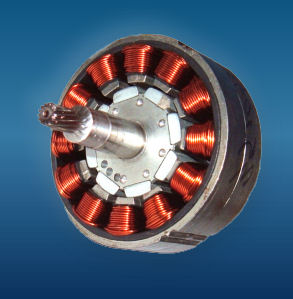
\includegraphics[width=2in]{images/bldc.jpg}
			\caption{Source: http://dev.emcelettronica.com/}
		\end{figure}
	\end{itemize}
}

\subsection{Shell Eco-Marathon}

\frame{
	\frametitle{Shell Eco-Marathon}
	
	\begin{itemize}
		\item Race for mileage, not speed
		\item Category:
		\begin{itemize}
			\item Urban Concept
			\item Protoype
		\end{itemize}
		\item plug-in electric
		\item 4 laps with 10 seconds stoppage between each lap
	\end{itemize}
}

\subsection{Problem Statement}
\frame{
	\frametitle{Problems}
	
	\begin{itemize}
		\item Types of torque produced by PMBLDC
		\begin{itemize}
			\item cogging torque
			\item reluctance torque
			\item mutual torque
		\end{itemize}
		
		\item Torque ripple
		
		\item Poor Strategy
	\end{itemize}
}
\subsection{Objectives}
\frame{
	\frametitle{Objectives}

	\begin{enumerate}
		\item To identify the output signal of the controller circuit and the hall effect sensor of the PMBLDC and develop a set of instrument for measuring the mileage of the electric vehicle.
		\item To study the track profile of Sepang North Track and create a simulation program for simulating the vehicle dynamics at the Sepang North Track.
		\item To compose a set of strategy to increase the mileage of the electric vehicle running on the Sepang North Track based using the simulation program.
	\end{enumerate}
}

\section{Methodology}
\frame{}

\section{Result}
\frame{}

\section{Conclusion}

\subsection{Conclusion}
\frame{}

\subsection{Future Work}
\frame{}

\end{document}
